\section{Introduction}

This chapter presents the description of the system created for this Bachelor's Thesis. The solution proposed implements a software capable of tracking the user's hands and learning and recognizing the objects that are hand-held. 
\\

The name of the proyect, OCULAR is an acronym of "On-line objeCt Learning And Recognition". The first word, on-line, refers to the fact that the learning of new objects is done in real time, there is no need of a training phase in which the software does not work. 
\\

\begin{figure}[h]
	\begin{center}
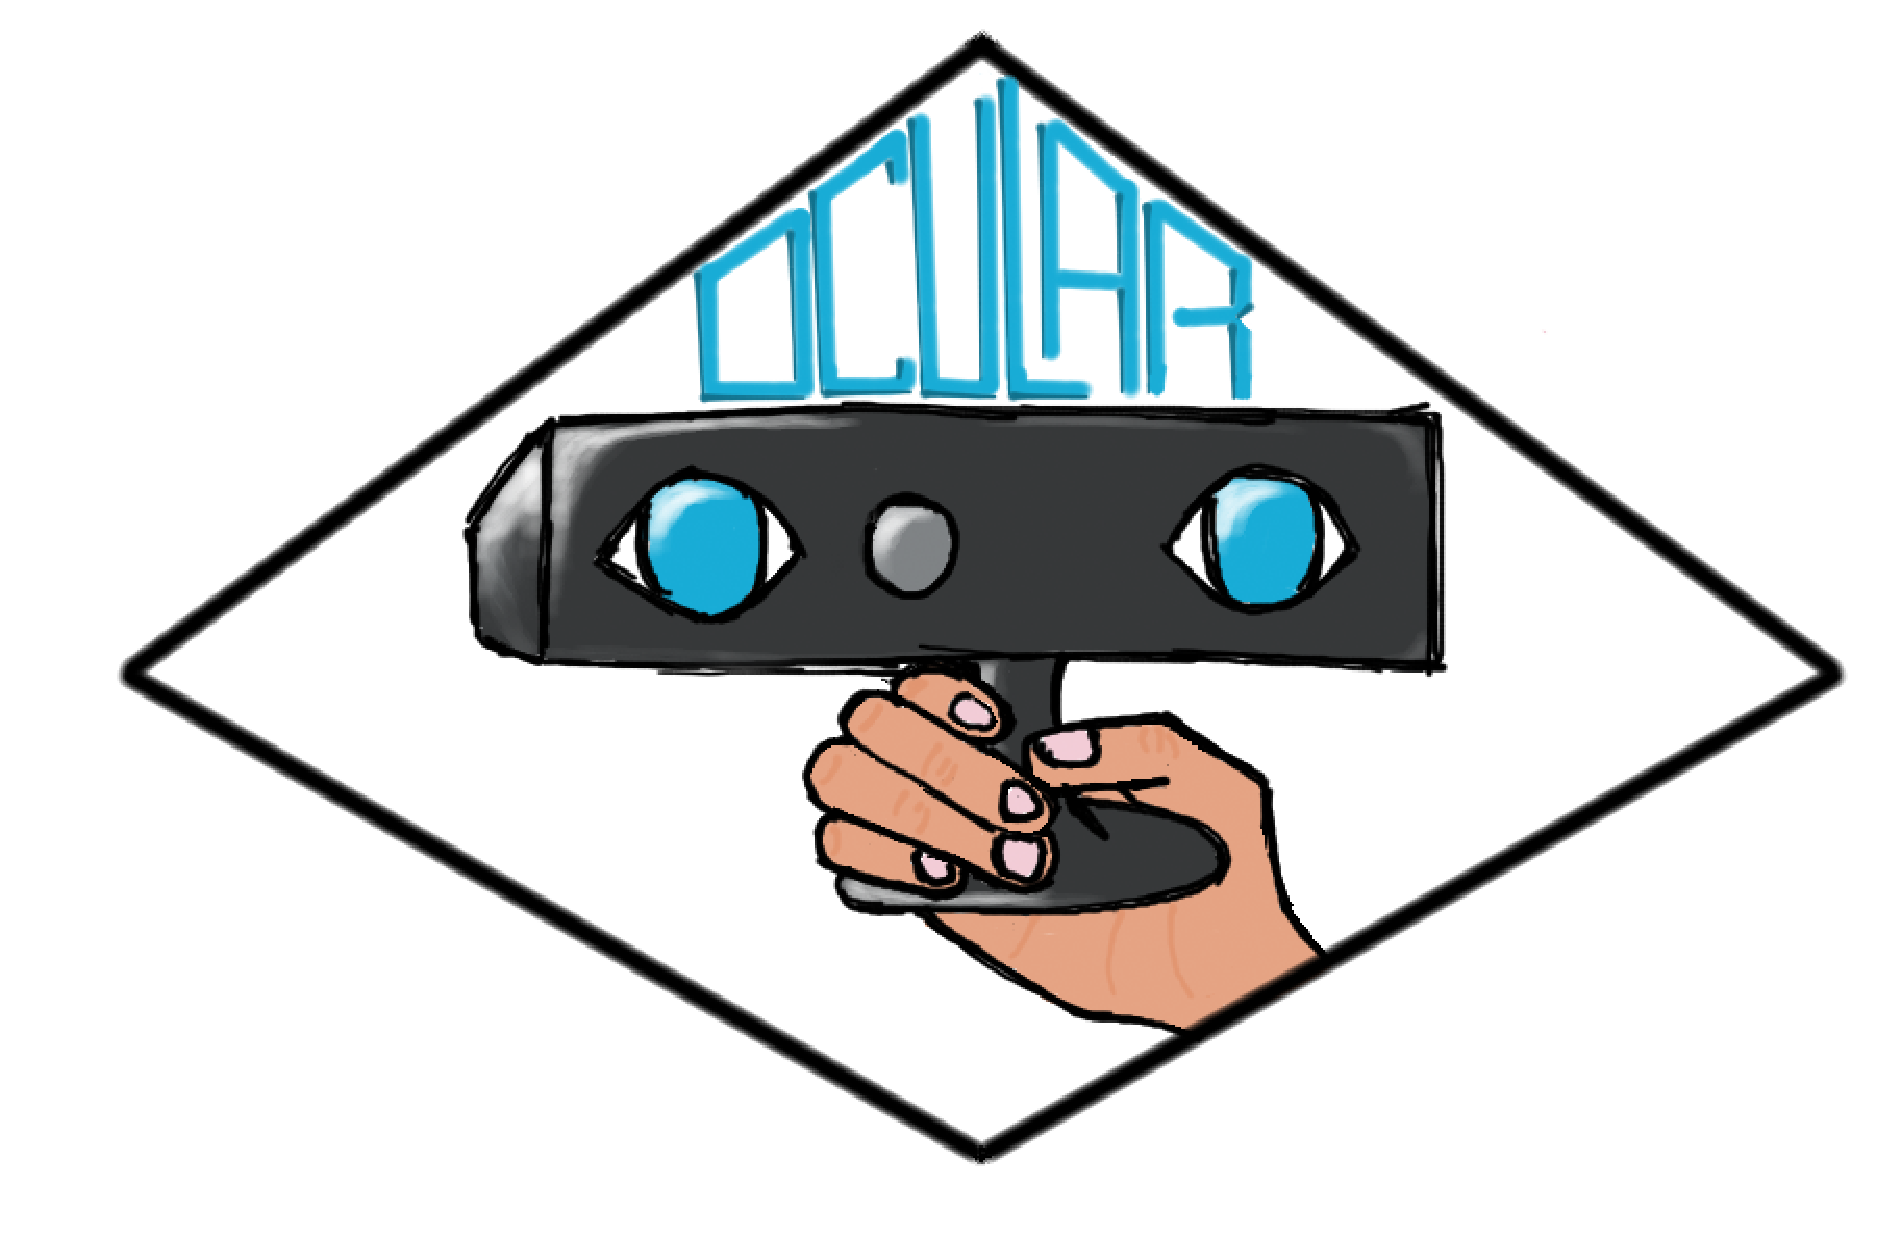
\includegraphics[scale=0.3]{img/ocular_logo.eps}
	\caption[OCULAR Logo]{OCULAR logo}
	\end{center}
\end{figure}

The project's software is modular and the processing has been distributed among different nodes. The ROS programming environment has been used in order to improve the communication between nodes and the overall performance of the code. The PCL and OpenCV C++ libraries has been included in the project in order to enhance the 3D and 2D data processing, respectively. 
\\
In the following section, the different design alternatives that appeared and the final chosen design are presented and explained.
